\section{Experiment 2: \textbf{search-shortsamples}}


Experiment 1 showed us that the visual system can effectively discriminate the complex patterns of motion and form found in fire, but cannot effectively search for them in longer video sequences. However, it only looked at test clips between 0.2 and 1 seconds in length.

In order to look at the discriminability and searchability of shorter clips, we performed Experiment 2. This study used an identical 2AFC delayed-match-to-sample technique, but with shorter video clips lasting between 0.02 and 0.24 seconds (1 to 12 frames at 50Hz).

\subsection{Methodology}


\paragraph{Stimuli}

A 1000-frame corpus of consecutive fire images was used.

\paragraph{Subjects}

12 subjects were recruited using a mailing list operated by University College London. All reported normal or corrected-to-normal vision.

\paragraph{Trial structure}

In each trial, a sample was presented first, followed by two tests. Subjects indicated which test they thought corresponded to the sample using the left arrow (first sample) and right arrow (second sample) keys. 

\paragraph{Factors}

Sample length (sL) was one of (1, 3, 6, 12) frames, 
equivalently (0.02, 0.06, 0.12, 0.24) seconds.

Test length was one of (15,20,40) frames, equivalently (0.3,0.4,0.8) seconds.

There were 3*4 = 12 conditions. We presented a total of 480 trials (40 trials per condition).

\paragraph{Block structure}

24 training trials were presented first.

Test length was varied across blocks. Sample length was varied within blocks.

We presented 3 blocks, one corresponding to each test length, in random order. Subjects took a short break between blocks.

\begin{figure}[H]
\centering
\renewcommand{\arraystretch}{1.8}

      \begin{subfigure}[b]{\textwidth}
\begin{tabular}{ >{\bfseries}r | p{8cm}   }
& \textbf{Experiment 2}\\
\hline
  
	Design & 2AFC delayed match-to-sample (sample clip followed by two test clips)\\                   
  Stimuli & 1000-frame corpus \\
  Factors & sample length: (0.02, 0.06, 0.12, 0.24) seconds or (1, 3, 6, 12) frames. \newline 
sample/test ratio: (0.3,0.4,0.8) seconds or (15,20,40) frames.\\
  Block design & Test length varied across blocks\newline
			Sample length varied within blocks \newline
			12 \newline
40 trials per condition \newline
600 trials \newline
25 training trials \\
\end{tabular}
\caption{Design summary.}
   \end{subfigure}

\begin{subfigure}[b]{\textwidth}
\centering
                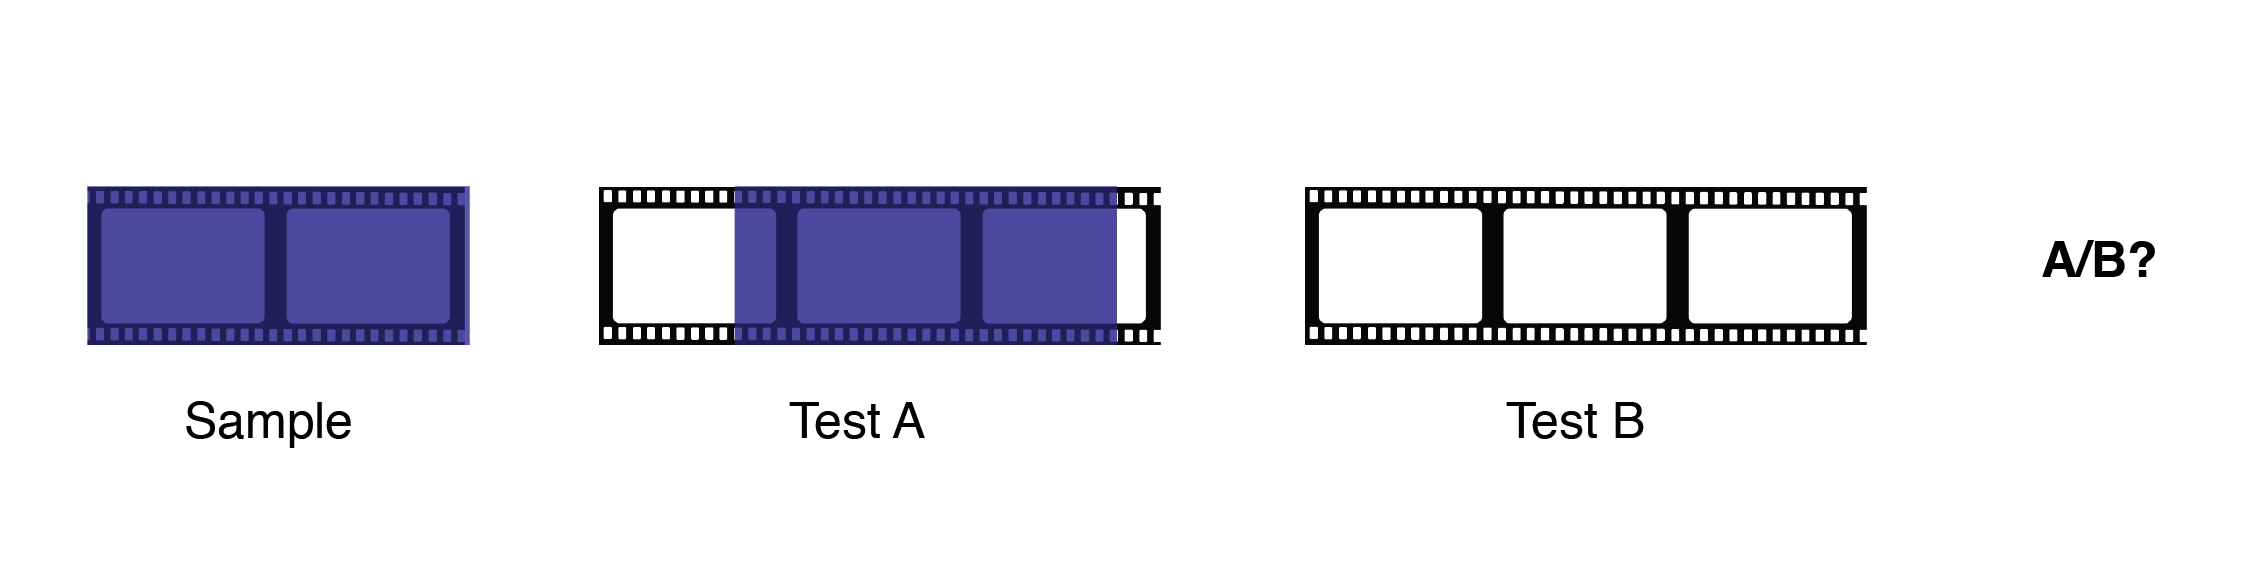
\includegraphics[width=12cm]{img/protocol_2afc.png}
                \caption{A short sample was followed by two longer tests, one of which contained the sample.}
         
        \end{subfigure}
\caption{Experiment 2: design summary and trial structure.}
\end{figure}

\subsection{Results}

\paragraph{Sample length}

Accuracy increased significantly with the length of the sample, and $t$-tests showed that it was always above chance across different sample lengths. Two-way repeated-measures ANOVA revealed a significant effect of sample length ($p<$0.00001), but not of test length ($p=$0.652), and no interaction between the two ($p<$0.395). Mean accuracies by target length were:


\paragraph{Learning}

As shown in Fig. \ref{f:e2:learn}, there is no discernible effect of learning during this task: subjects' accuracy did not improve during the first 100 trials, as in Experiment 1. It is tempting to explain this result by the fact that Experiment 1 kept sample lengths constant within blocks, allowing subjects to tune their mental set to a particular sample length. However, Experiment 1 used 3 blocks of 200 trials each, and we note no drop in accuracy after the end of the first or second block. We thus conclude that the lack of learning is related to the shorter sample lengths.

\begin{center}
\begin{tabular}{ r | l   }
\textbf{Sample length} & \textbf{Mean accuracy}\\
\hline
0.02 s &  0.6\\
0.06 s&  0.67\\
0.12 s& 0.70\\
0.24 s&  0.73\\
\end{tabular}
\end{center}

\begin{figure}[htp]
\centering
\begin{subfigure}[b]{\textwidth}
\centering
                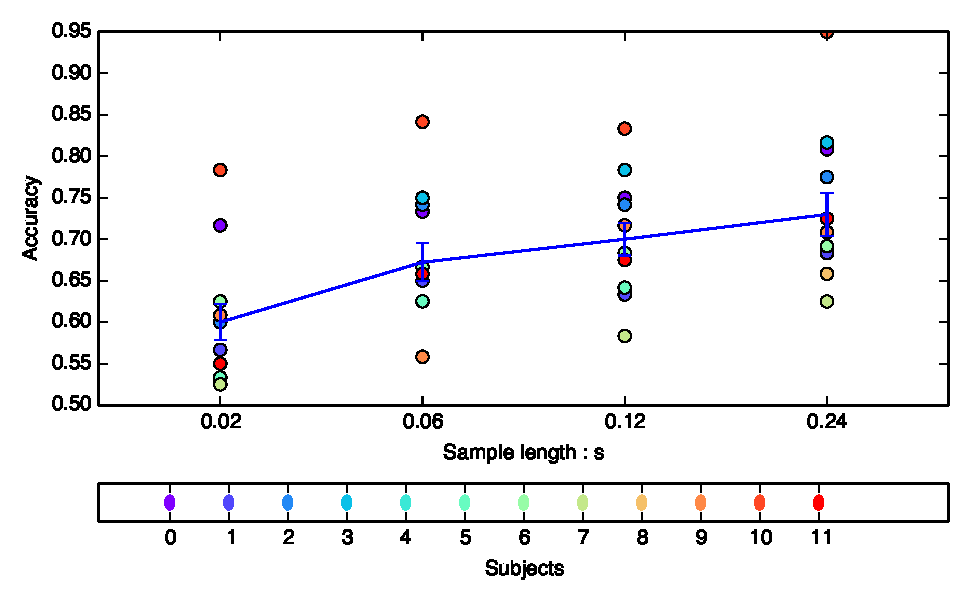
\includegraphics[width=12cm]{img/fig_fire4_correct_sampleL.pdf}
                \caption{Accuracy against sample length. Longer samples are easier to match.}
          
        \end{subfigure}
\begin{subfigure}[b]{\textwidth}
\centering
                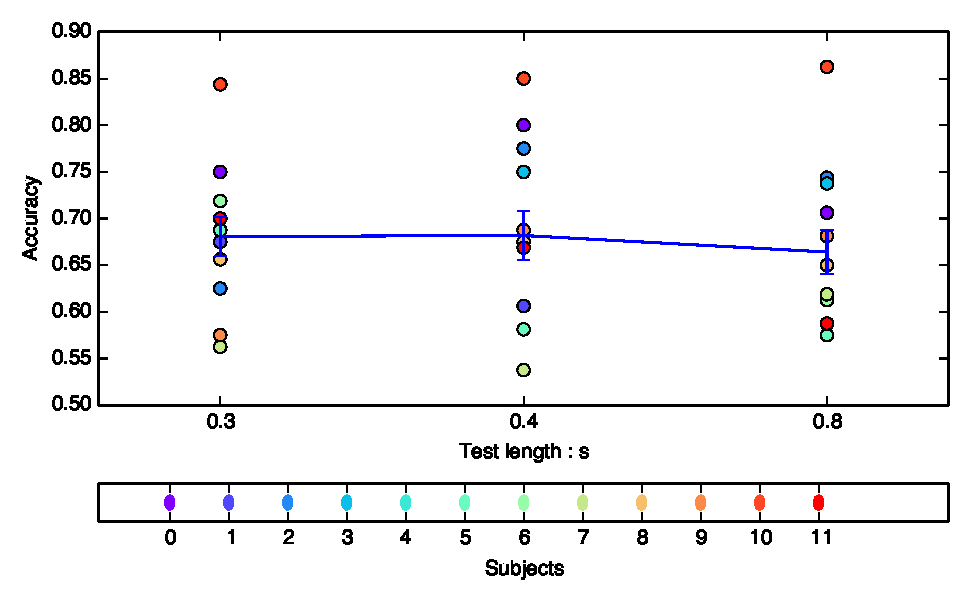
\includegraphics[width=12cm]{img/fig_fire4_correct_testL.pdf}
                \caption{Accuracy against test length. Search for samples under 0.24 seconds is not affected by test length.}
         
        \end{subfigure}
\caption{Experiment 2: For samples under 0.24 seconds, search is more effective with longer samples; however, test length makes no difference up to 0.8 seconds.}
\end{figure}

\begin{figure}[htb]
\centering
\begin{subfigure}[b]{\textwidth}
\centering
                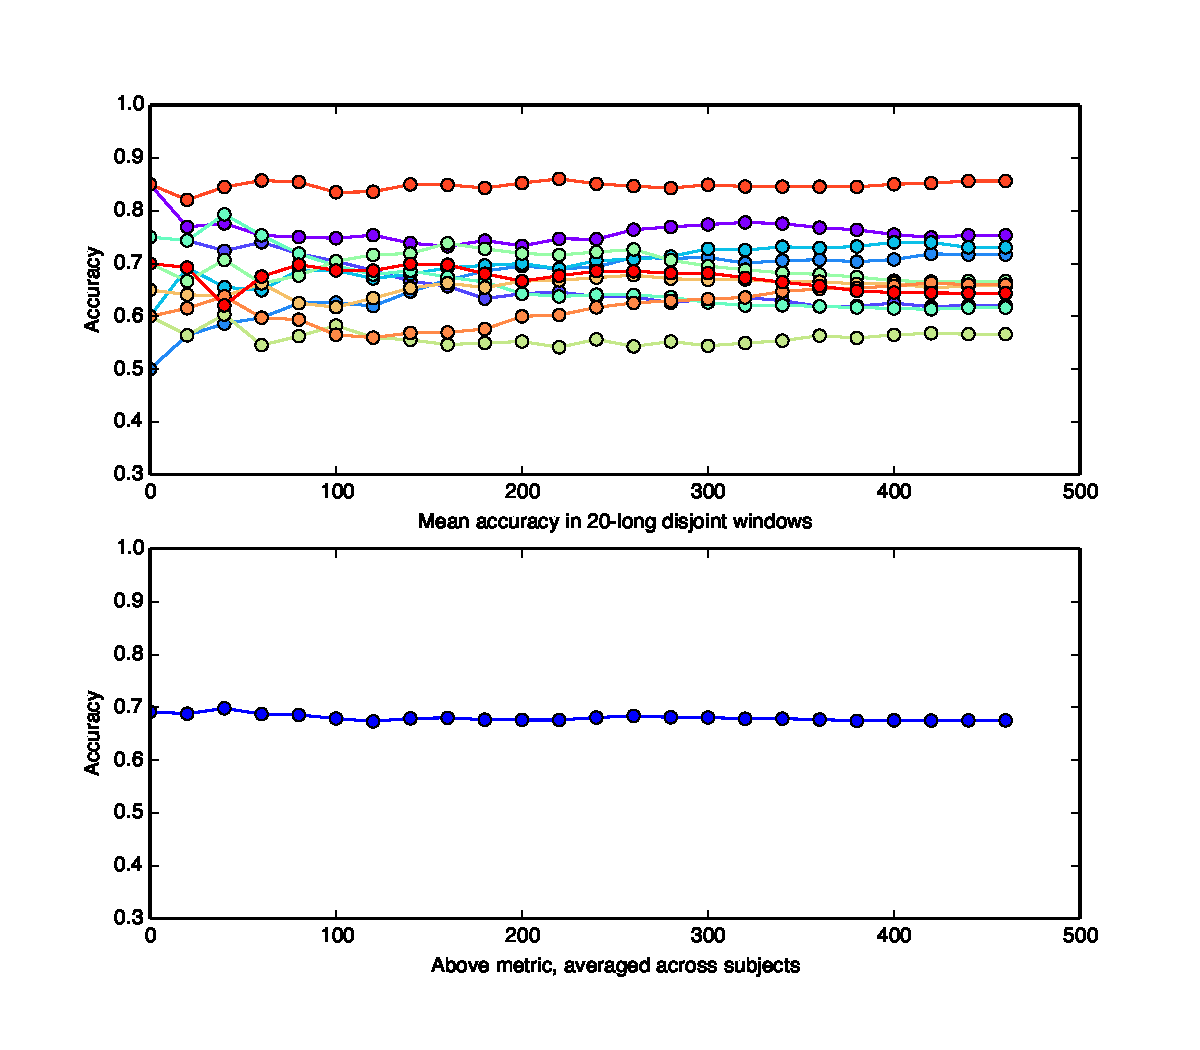
\includegraphics[width=12cm]{img/fig_fire4accuracyWalkingWindow.pdf}
                \caption{Learning: accuracy vs. trial number, blocked into groups of 20.}
      		\label{f:e2:learn}
        \end{subfigure}
\caption{Experiment 2: for short samples under 0.24 seconds, there is no discernible effect of learning.}
\end{figure}

\subsection{Discussion}